\needspace{8.2cm}\noindent\begin{minipage}[t]{3.1cm}\vspace{0pt}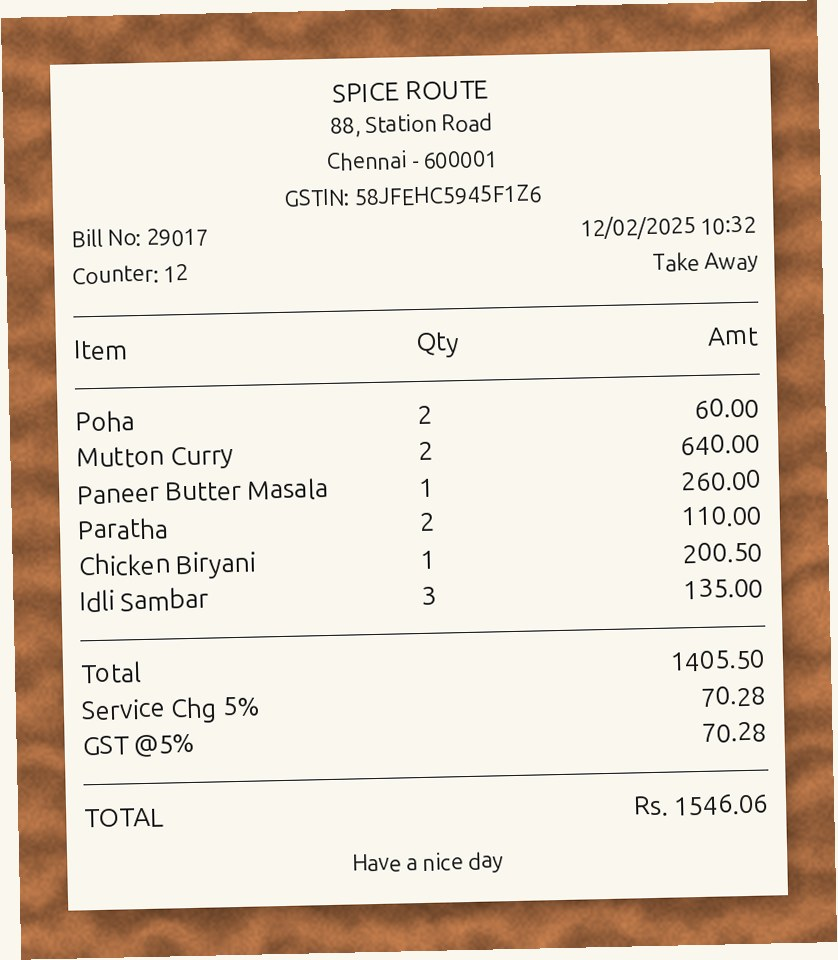
\includegraphics[width=3.1cm]{../examples/final_run/final_017.jpg}\end{minipage}\hfill
\begin{minipage}[t]{\dimexpr\linewidth-3.4cm\relax}\vspace{0pt}{\footnotesize\renewcommand{\arraystretch}{1.0}
\textbf{Bill 3.} The model read 6 items and 2 charges. Corrections made on the check screen: none needed.\\[2pt]
\begin{tabular}{@{}lrrrr@{}}\toprule & Riya & Aman & Sara & Bill\\\midrule
Poha & 20.00 & 20.00 & 20.00 & 60.00 \\
Mutton Curry & 426.67 & 213.33 & 0.00 & 640.00 \\
Paneer Butter Masala & 0.00 & 0.00 & 260.00 & 260.00 \\
Paratha & 110.00 & 0.00 & 0.00 & 110.00 \\
Chicken Biryani & 0.00 & 200.50 & 0.00 & 200.50 \\
Idli Sambar & 0.00 & 67.50 & 67.50 & 135.00 \\
\midrule
Service Charge & 27.83 & 25.07 & 17.38 & 70.28 \\
GST & 27.83 & 25.07 & 17.38 & 70.28 \\
\midrule
Total (Rs) & \textbf{612.33} & \textbf{551.47} & \textbf{382.26} & \textbf{1546.06} \\
\bottomrule\end{tabular}\\[2pt]
\textit{Sara: Poha (1/3 share, Rs 20.00) + Paneer Butter Masala (full, Rs 260.00) + Idli Sambar (1/2 share, Rs 67.50) = Rs 347.50 pre-tax subtotal. Sara's pre-tax subtotal is 24.7\% of the Rs 1405.50 of items on the bill, so Sara carries 24.7\% of each tax, service charge, discount and rounding line. ...}}\end{minipage}
\par\vspace{5pt}
